\documentclass[11pt]{article}
\usepackage{graphicx}
\usepackage{wrapfig}

\title{Data collection}
\author{Karl Menzel}

\begin{document}

\maketitle

\section{Data Collection}
The data is an updated version of the data used in Weber et. al. (2013). This data was requested by Anna Ritz in the early fall of 2016.The data is held in two files BadgerInfo.txt and BadgerMatrix.txt.
\begin{itemize}
\item \textbf{BadgerInfo.txt}  This contains demographic information about the badgers in in the study.  It contains four columns: badger name, sex,whether or not they are infected with tuberculosis, and the social group the badger is a part of.

\item  \textbf{BadgerMatrix.txt}  This contains the interaction data of the badgers. This matrix is constructed as usual with each cell being the interaction between the row and column badger.  The number in the cell denotes the amount of time that the two badgers were in close contact
\end{itemize}

\begin{wrapfigure}{h!}{.5\textwidth}
%\centering % center the figure
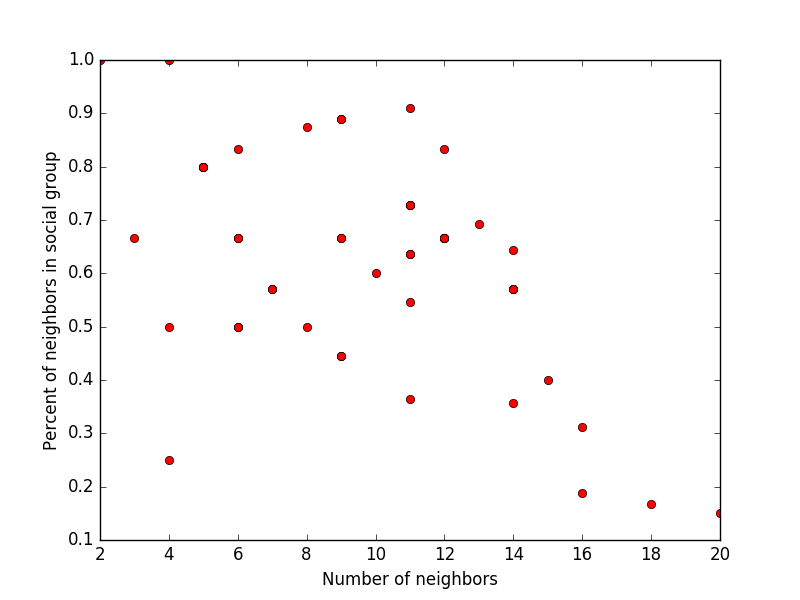
\includegraphics[width=\linewidth]{proportionInOut.png}
\caption{the number of neighbors by the number proporiton of neighbors in the same social group.} % caption
\label{figure} % add a label to reference it
\end{wrapfigure} 
 
\section{Summary Statistics}
This data consists of all of the interactions of 52 badgers.  This population of badgers consists of 9 social groups which are defined by the setts (tunnel system) where they live.  Following are statistics that represent the proportion of these interaction that are between members of the same social group and between members that are not in the same social group as well as aggregates for each social group.  In table \ref{table} Number of Edges on Nodes in Group is found by $|(i,j) : (i,j) \in E$ and $  i \in S_i| $ given nodes i and j in graph G = (V,E) and social group S and the next column is the proportion of those edges that had one edge outside the social group.  In figure \ref{figure} we see the number of neighbors on the x-axis and the proportion of neighbors in social group given as $\frac{|j: (i,j) \in E, S_j \neq S_i |}{|j: (i,j) \in E| }$ given two nodes (i and j) in graph G = (V, E) with social groups S on the y-axis.


\begin{table}[h]
\centering
\label{table}
\caption{Summary of whether edges that start in a social group end in the same social group or another social group.}
\begin{tabular}{| c | c | c  | }
\hline
Group & Number of Edges On Nodes in Group & Proportion of Internal Edges\\
\hline
1 & 109 & 0.660550458716 \\
\hline
3 & 44 & 0.545454545455 \\
\hline
2 & 9 & 0.666666666667 \\
\hline
5 & 60 & 0.2 \\
\hline
4 & 41 & 0.487804878049 \\
\hline
7 & 76 & 0.526315789474 \\
\hline
6 & 27 & 0.740740740741 \\
\hline
8 & 128 & 0.71875\\
\hline
\end{tabular}
\end{table}











\end{document}